\documentclass[12pt]{article}
\usepackage{graphics}
\usepackage{graphicx, verbatim}
\usepackage{amssymb}
\usepackage{amsmath}
% \usepackage[T1]{fontenc}
% \usepackage[utf8]{inputenc}
\usepackage{authblk}
\textwidth=6.2in
\textheight=8.5in
%\parskip=.3cm
\oddsidemargin=.1in
\evensidemargin=.1in
\headheight=-.3in

\usepackage{Sweave}
\begin{document}
\Sconcordance{concordance:modelNotes.tex:modelNotes.Rnw:%
1 14 1 1 0 36 1}



%To put figures in subfolder
%\SweaveOpts{prefix.string=figures/fig}
\DefineVerbatimEnvironment{Sinput}{Verbatim} {xleftmargin=2em}
\DefineVerbatimEnvironment{Soutput}{Verbatim}{xleftmargin=2em}
\DefineVerbatimEnvironment{Scode}{Verbatim}{xleftmargin=2em}

\title{\LARGE How coexistence mechanisms mediate temporal stability}
\author[1]{\large Andrew T. Tredennick}
\author[1]{\large Peter B. Adler}
\author[2]{\large Frederick Adler}
\affil[1]{\footnotesize Department of Wildland Resources and the Ecology Center, Utah State University}
\affil[2]{\footnotesize Departments of Biology and Mathematics, University of Utah}
\maketitle

%----------------------------------------------------
\section{\large Introduction}
%----------------------------------------------------
Theoretical work aimed toward identifying the mechanisms by which species richness promotes temporal stability has treated species coexistence as a foregone conclusion. In so doing, that large body of work implicitly assumes that the interaction between environmental variability and the mechanism(s) by which species coexist is trivial. However, under the same conditions of environmental variability, population dynamics will respond differently depending on the coexistence context. In turn, this leads to different dynamics at the community and ecosystem levels depending on how species interact. So, it stands to reason that identifying the key mechanisms that promote ecosystem stability requires a solid understanding of how species coexistence mediates temporal stability in fluctuating environments.

To that end, we will analyze a general consumer-resource model under different coexistence assmptions. Our starting point is a model of two plant consumers and one resource (e.g., soil moisture or nitrogen). We will focus on four cases of species coexistence:
\begin{enumerate}
  \item Relative nonlinearty
  \item Storage effect with exploitative competition only (e.g., `temporal storage effect')
  \item Storage effect with interference competition only (e.g., `spatial storage effect')
  \item A combination of all three mechanisms
\end{enumerate}

Each scenario requires different model assumptions and structure, so we will describe each in turn. Although the structure may change slightly to incorporate different coexistence mechanisms, the strength of our approach lies in the similarities among the models since we work under a unified consumer-resource framework.

\subsection{A general consumer-resource model}
We start with a general consumer-resource model where the consumer can be in one of two-states: a dormant state $D$ and a live state $N$. Transitions between $N$ and $D$ occur at discrete intervals $T$, so our model is formulated as ``pulsed differential equations". For clarity we refer to $T$ as years and the growing time between years, $\tau$, as seasons. Seasonal (within-year) dynamics are modeled as three differential equations:
\begin{align}
\frac{\text{d}D_{i}}{\text{d}\tau} &= -(m_{D,i}D_{i})\\
\frac{\text{d}N_{i}}{\text{d}\tau} &= f(R)N_{i} - m_{N,i}\\
\frac{\text{d}R_{i}}{\text{d}\tau} &= a(S - R) - \sum\limits_{i=1,2}f(R)N_{i}
\end{align}
where $i$ denotes species, $D$ is the dormant (long-lived) biomass state, $N$ is the living biomass (fast-growing, shorter-lived) state, and $m$s are biomass loss rates. The growth rate of living biomass is a resource-dependent function, $f(R) = r_{i}R/(K_{i}+R)$, where $r$ is the maximum growth rate and $K$ is the resource level at which growth is one-half $r$. For the resource dynamics, whose state is denoted by $R$, we use a linear resource renewal equation where $a$ scales resource turnover rate and $S$ is the resource equilibrium when consumers are absent, and an offtake of the resource equal to the sum of each species' consumption, $\sum_{i=1,2}f(R)N_{i}$. Note that since transitions between $N$ and $D$ are pulsed, only biomass loss occurs throughout the season for $D$.

At the beginning of each season we start with initial conditions defined as $V_{t}$, $W_{t}$, and $Z_{t}$ for the dormant state, the live state, and the resource, respectively. So for each season, Eqs. 1-3 are solved given the initial conditions:
\begin{align}
  D_{i}(0) &= V_{i,t} \\
  N_{i}(0) &= W_{i,t} \\
  R(0) &= Z_{t}
\end{align}
The consumers transition between $N$ and $D$ instantaneously between years. We assume resource density does not change between years. So, at the yearly transition:
\begin{align}
  V_{i,t+1} &= D_{i}(T^-) + N_{i}(T^-) - D_{i}(T^-)g_{t} \\
  W_{i,t+1} &= D_{i}(T^-)g_{t} - N_{i}(T^-) \\
  Z_{t+1} &= R(T^-)
\end{align}
where $D(T^-)$, $N(T^-)$, and $R(T^-)$ are the densities of each state at the end of the year and $g$ is a time-fluctuating activation rate that regulates how much dormant biomass is converted to growing-season live biomass each year. Our formulation assumes that at the end of each season all accumulated living biomass [$N(T^-)$] is converted to dormant biomass.

\subsubsection{Implementing the storage effect}
To make this a ``storage-effect" model, we need to satisfy three conditions: (1) the organisms must have a mechanism for persistence under unfavorable conditions, (2) species must respond differently to environmental conditions, and (3) the effects of competition on a species must be more strongly negative in good years relative to unfavorable years. Our model meets condition 1 because we include a dormant stage with very low death rates. We satisfy condition 2 with our model whenever $g$ is not perfectly correlated between species. Lastly, our model meets condition 3 because condition 2 partitions intraspecific and interspecific competition into different years. Thus, during a high $g$ year for one species, resource uptake is also inherently high for that species, which increases intraspecific competition relative to interspecific competition. So, given adequate variability in $g$, the inferior competitor (species with lower $r$) can persist.  

\begin{figure}
\begin{center}
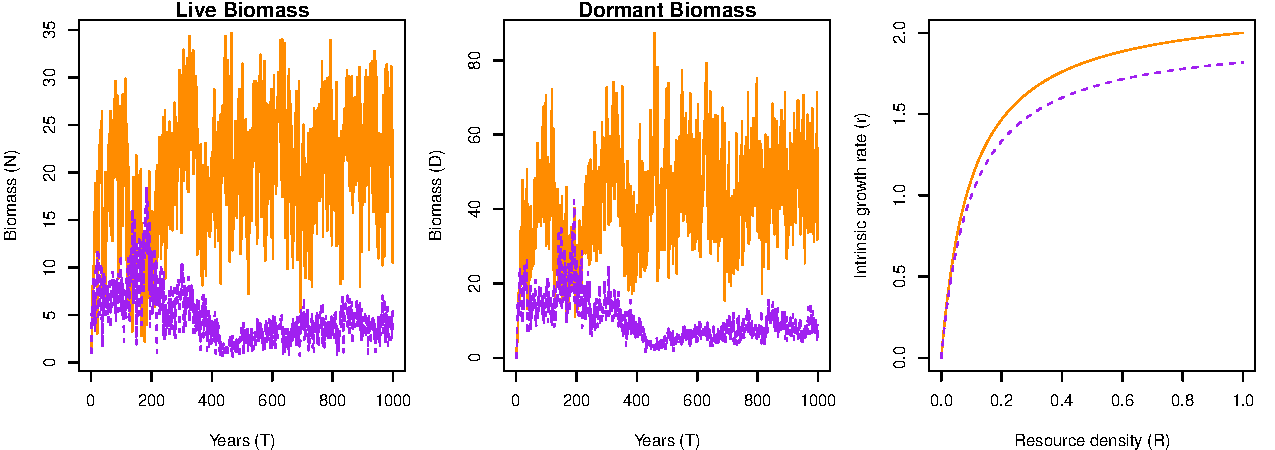
\includegraphics{Fig-001}
\end{center}
\caption{Example time-series from our pulsed consumer-resource model where $g$ is perfectly uncorrelated, $r_1$ = r[1], and $r_2$ = r[2]. Species 1 is orange, species 2 is purple. The far right panel shows how the growth rates of the two species change with resource density (this becomes important when modeling relative nonlinearity).}
\end{figure}


\end{document}
